\documentclass[10pt, onecolumn]{article}
\usepackage[margin=1in]{geometry}
\usepackage{lmodern}% http://ctan.org/pkg/lm
\usepackage{authblk} % adds affiliations

\usepackage[utf8x]{inputenc}
\usepackage{nameref}
\usepackage[right]{lineno}
\usepackage{amsmath}
\usepackage{booktabs}
\usepackage[numbers,super]{natbib}
\usepackage{changepage}

% adjust caption style
\usepackage[aboveskip=1pt,labelfont=bf,
            labelsep=period,singlelinecheck=off]{caption}

% remove brackets from references
\makeatletter
\renewcommand{\@biblabel}[1]{\quad#1.}
\makeatother

\usepackage[colorinlistoftodos]{todonotes}

% headrule, footrule and page numbers
\usepackage{lastpage,fancyhdr,graphicx}
\usepackage{epstopdf}
\pagestyle{myheadings}
\pagestyle{fancy}
\fancyhf{}
\rfoot{\thepage/\pageref{LastPage}}
\renewcommand{\footrule}{\hrule height 2pt \vspace{2mm}}

% use \textcolor{color}{text} for colored text (e.g. highlight to-do areas)
\usepackage{color}

\definecolor{Gray}{gray}{.25}

\usepackage{graphicx}

% use if you want to put caption to the side of the figure
\usepackage{sidecap}

\usepackage{xcolor}
\usepackage[colorlinks = true,
            linkcolor = blue,
            urlcolor  = blue,
            citecolor = blue,
            anchorcolor = blue]{hyperref}

% ####################################################
% ####################################################
% ####################################################
\usepackage[colorinlistoftodos]{todonotes}
% ####################################################
% ####################################################
% ####################################################





% use for have text wrap around figures
\usepackage{wrapfig}
\usepackage[pscoord]{eso-pic}
\usepackage[fulladjust]{marginnote}
\reversemarginpar{}

\usepackage{gensymb}
\usepackage{siunitx}

% new commands
% q value
\newcommand{\qval}[1]{$q<10^{-#1}$}

% species names
\newcommand{\cel}{\emph{C.~elegans}}
\newcommand{\dicty}{\emph{D.~discoideum}}
\newcommand{\ecol}{\emph{E.~coli}}
\newcommand{\gf}{gain-of-function allele}
\newcommand{\lf}{loss-of-function allele}
\newcommand{\strong}{strong loss-of-function allele}
\newcommand{\weak}{weak loss-of-function allele}


% gene names
% \newcommand{\gene}[1]{\emph{#1}} # for MS word typesetting
\newcommand{\gene}[1]{\mbox{\emph{#1}}}
\newcommand{\genotype}[1]{\mbox{\emph{#1}}}
\newcommand{\protein}[1]{\mbox{\uppercase{#1}}}
\newcommand{\ras}{\gene{let-60} (\emph{ras})}
\newcommand{\rasp}{\protein{let-60}}
\newcommand{\dpy}{\gene{dpy-22} (\emph{med-12})}
\newcommand{\letgfn}{3,021}
\newcommand{\letlfn}{857}
\newcommand{\letgf}{\gene{let-60(gf)}}
\newcommand{\letlf}{\gene{let-60(lf)}}
\newcommand{\strongn}{2,821}
\newcommand{\weakn}{434}
\newcommand{\transn}{2,930}

% protein names

% DE genes numbers:

% downstream targets

% website commands


% more space between rows
\newcommand{\ra}[1]{\renewcommand{\arraystretch}{#1}}

\title{A study of allelic series using transcriptomic phenotypes}

\author[1,2]{David Angeles-Albores}
\author[1,2,*]{Paul W. Sternberg}
\affil[1]{Division of Biology and Biological Engineering, Caltech,
Pasadena, CA, 91125, USA}
\affil[2]{Howard Hughes Medical Institute, Caltech, Pasadena, CA, 91125, USA}
\affil[*]{Corresponding author. Contact: pws@caltech.edu}
\renewcommand\Affilfont{\itshape\small{}}

% document begins here
\begin{document}
% title
\maketitle

\section*{Abstract}

\textbf{
Abstract goes here
}

\vspace{10mm}

\section*{Significance Statement}


\vspace{10mm}

\linenumbers{}

\section*{Introduction}
Allelic series refers to the study of alleles with different phenotypes in order
to understand the molecular properties that this locus controls. Allelic series
are historically important for genetics. Indeed, the earliest authors to use the
term `allelic series' are Barbara McClintock~\cite{} and Elizabeth S.
Russell~\cite{}. In her work, McClintock studied a deficiency of the tail end of
chromosome 9 of maize by generating trans-heterozygotes with mutants of various
genes that she knew existed near the end of chromosome 9. Her work allowed her
to infer that the deficiency was modular, effectively generating a double mutant
that behaved as a single allele but which could participate phenotypically in
two distinct allelic series. From this study, McClintock made inferences about
the role of large deletions in generating null mutants and the modifying effects
of placing a loss-of-function mutation in \emph{trans} to a deficiency or large
deletion. In multiple senses, this work precluded later observations in yeast
that showed two mutant alleles of the same genetic unit, when placed in
\emph{trans} to each other, could complement and generate a wild-type phenotype.
Allelic series have also been used to study the dose response curve of a
phenotype for a particular gene. In \cel{}, the \gene{let-23} allelic series
stands out as an example~\cite{}.

As case studies, we focus on an allelic series of the \gene{let-60} gene and an
allelic series of the \gene{dpy-22} gene in \cel{}. \gene{let-60} is the
\gene{ras} orthologue in \cel{}~\cite{Han1990a}, where it functions to promote
the cellular fate of a number of cells during development~\cite{Yochem1997}.
\ras{} is a GTPase~\cite{Han1990a} that cycles between GDP- and GTP-binding
states. The GTP-binding state is considered to be the signaling
competent state. \gene{dpy-22} is the \gene{med-12} orthologue in
\cel{}~\cite{}\todo{cite}.

In \cel{}, \ras{} always acts downstream of a receptor\todo{citation}. Activated
\ras{} can activate signaling cascades to transmit information to the eukaryotic
nucleus. Often, this signaling cascade consists of \gene{lin-45} (the RAF
ortholog)~\cite{Han1993a}, \gene{mek-2}~\cite{Wu1995} and
\gene{mpk-1}~\cite{Lackner1994}. The Ras pathway has been extensively studied in
the context of vulval organogenesis, where it acts downstream of
\gene{let-23}~\cite{Sternberg1995} to promote vulval induction of the
P\emph{n}.p cells. In addition to vulval development, \ras{} has been implicated
in the migration of the Sex Myoblasts (SM), where it acts both cell autonomously
and non-autonomously, the formation of the excretory pore, hypodermal fluid
homeostasis, as well as germline development and the formation of the male
tail~\cite{Sundaram2006}. Thus, the Ras pathway is pleiotropic, but its
phenotypes are separable and specific.

The intense scrutiny of the Ras pathway has led to the generation of a large
number of loss-of-function alleles for \ras{}. Null mutations of \ras{} are
known to be lethal, but reduction-of-function alleles have been useful to
carefully dissect the molecular properties of this protein. Gain-of-function
mutations of \ras{} are also known, although they are much more rare. In
particular, a single gain-of-function mutation, \emph{n1046gf}, was famously
isolated multiple times in several
screens~\cite{Han1990,Beitel1990a,Ferguson1985} leading to a Multivulva (Muv)
phenotype. \todo{Is Ferguson 1985 the right citation here} These
gain-of-function mutations have a privileged history in the Ras pathway, as they
have been used in multiple screens to identify genes that have a Suppressor of
Ras (Sur) phenotype \todo{anything else that I need to cite here?} such as
\gene{sur-1} (now \gene{mpk-1}~\cite{Lackner1994}) or
\gene{sur-2}~\cite{Singh1995}. Interestingly, although nulls of these genes are
often lethal, strong loss-of-function alleles can be obtained for these
suppressors. Moreover many of these suppressor alleles have no phenotype in a
wild-type background~\cite{}. This suggests that many of these genes mediate
very little Ras signaling under most situations yet have significant dynamic
range in the amount of signaling they can accomodate.

Talk about \gene{dpy-22}.

In this paper, we set out to sequence a weak gain-of-function (\emph{n1046gf})
and a strong loss-of-function (\emph{n2021}) allele of Ras, as well as a weak
loss-of-function (\emph{bx93}) and a strong-loss-of-function (\emph{sy622})
allele of \dpy{}. In either allelic series we found behaviors that challenge the
way we think about alleles and allelic series.


\section*{Results}
\subsection*{Comparing \emph{ras(gf)} and \emph{ras(lf)} alleles}
As a first survey of allelic series, we sequenced in triplicate two alleles of
\gene{let-60}, \gene{let-60(n1046gf)} and \gene{let-60(n2021)} at the young
adult stage and compared them with wild-type samples at the same stage. We
sequenced each sample at a depth of 20M reads. These reads were pseudo-aligned
using Kallisto~\cite{}, which allowed us to quantify 21,800 protein-coding
isoforms. After quantification, we performed differential expression analysis
using Sleuth~\cite{}. Briefly, Sleuth uses a General Linear Model to identify
genes that are differentially expressed by log-transforming the estimated counts
of a given isoform in all the samples and performing a linear regression between
a given mutant and wild-type. The slope of the linear regression, $\beta$, is a
measurement of the magnitude of the perturbation, loosely analogous to the
natural logarithm of the fold-change (see Angeles-Albores \emph{et al}~\cite{},
Figure 1). These slopes are tested against the null hypothesis that they are
equal to zero. An isoform is considered to be differentially expressed when the
$q$-value ($p$-value corrected for false discovery rate) is less than 0.1.
$\beta$ values can be positive or negative---positive values of $\beta$ indicate
an isoform that is up-regulated in the mutant relative to the wild-type control,
whereas negative values of $\beta$ indicate an isoform that is down-regulated in
the mutant relative to the wild-type control. When we refer to $\beta$ and
$q$-values, it will always be in reference to isoforms. However, when speaking
about the size of a gene set, we will always quantify it as the number of
individual genes contained in the set. For \cel{}, the difference between the
number of isoforms and genes is negligible because most protein-coding genes
have a single isoform.


We predicted that the transcriptomes of these alleles
would show the same set of differentially expressed genes (henceforth referred
to them as a shared transcriptomic phenotype, STP) because these alleles are
both perturbing the GTP-binding potential of the protein product. Moreover, we
predicted genes within this STP would show weaker perturbations on average
within one mutant compared to the other.
We identified \letgfn{} differentially expressed genes in the \letgf{} mutant
relative to the wild-type control, and \letlfn{} differentially expressed genes
in the \letlf{} mutant relative to the wild-type control (see
Fig.~\ref{fig:rasplots}).

Contrary to our expectations, the STP between these two alleles consisted of
31\% of the differentially expressed genes in the \letlf{} transcriptome,
totalling 269 genes. Moreover, we found that this STP showed a strong positive
correlation between the two alleles. In order to assess whether one allele was
significantly stronger than another we split the STP into its correlated and
anti-correlated components and found the regression line in each component. We
measured a correlation coefficient of 1.03 and -1.00 for each component,
indicating that the two alleles have effects that are exactly opposite on
average. Our results suggest the existence of four phenotypes: A phenotype
associated exclusively with \letgf{} (the \letgf{}-specific phenotype), another
associated exclusively with \letlf{} (the \letlf{}-specific phenotype), a
phenotype that is the dpy-6 in both alleles and a phenotype that is inverted in
one allele relative to the other.

\begin{figure}
  \centering{}
  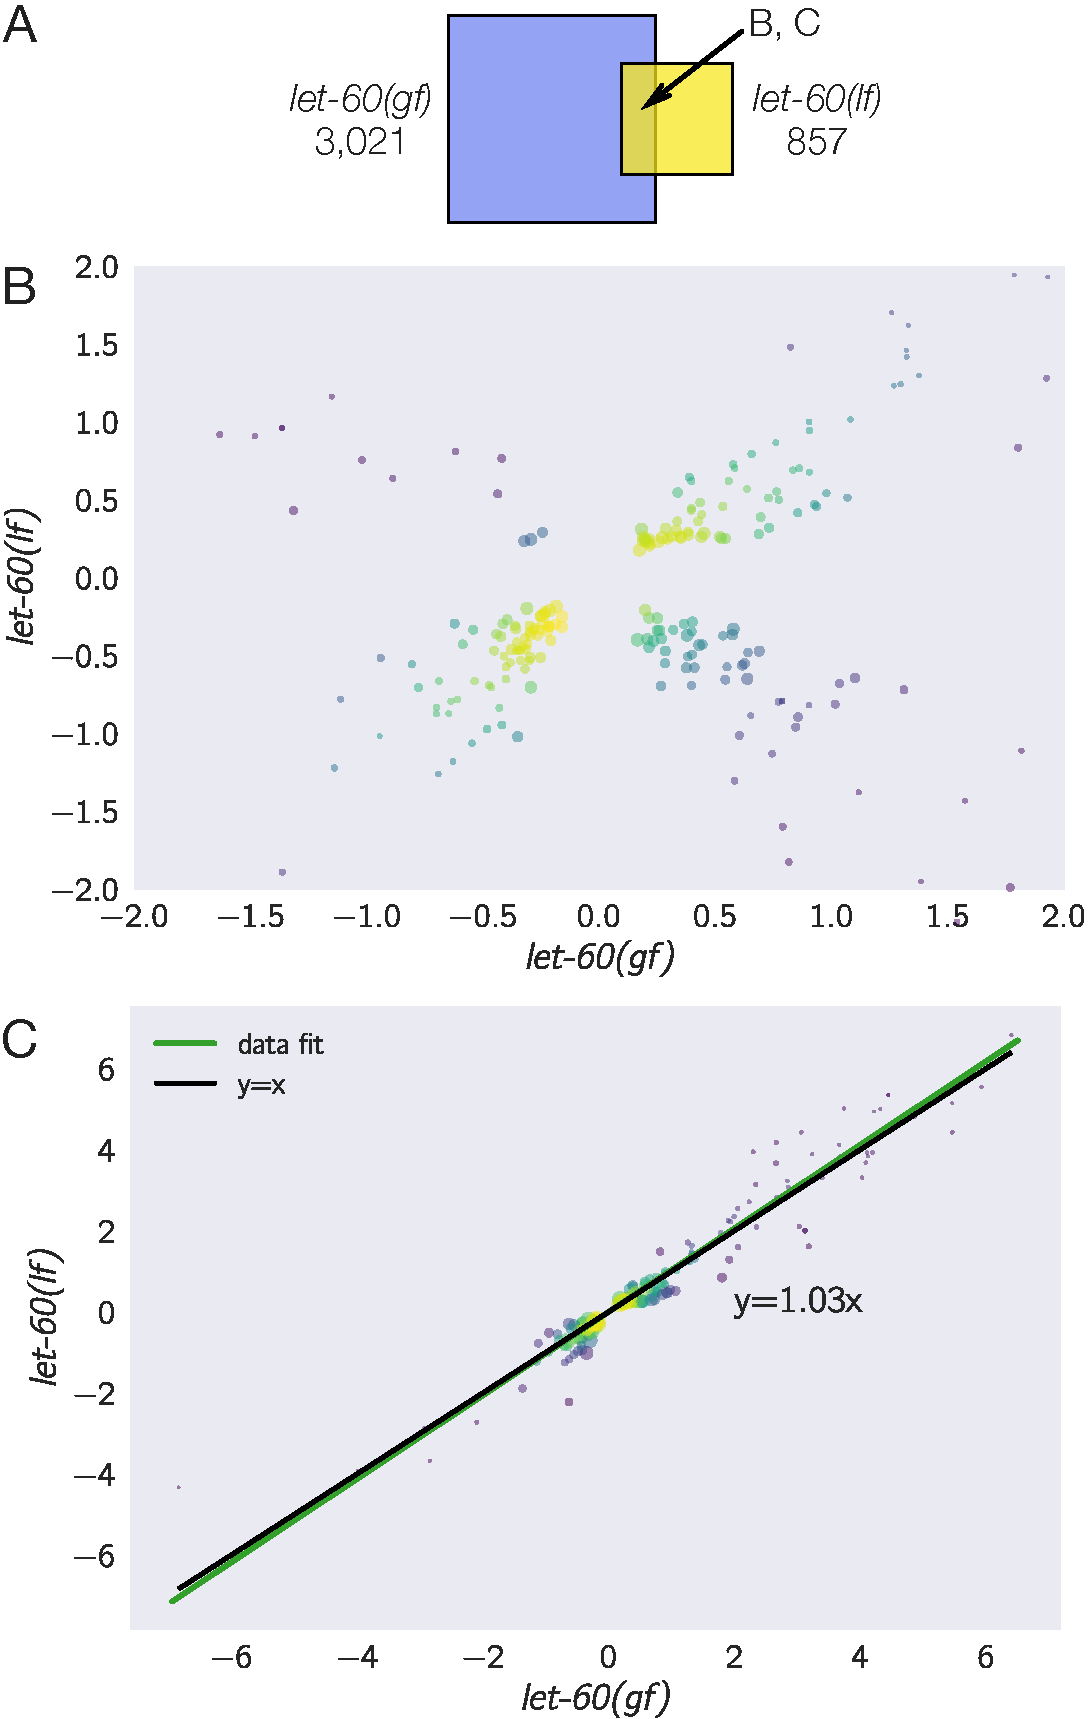
\includegraphics[width=0.5\textwidth]{../figs/ras_allele_plots.pdf}
  \caption{
    \textbf{A}. Venn diagram of the differentially expressed genes in a \letgf{}
    and a \letlf{} mutant. Diagram is to scale.
    \textbf{B}. $\beta$ coefficients for isoforms that are differentially
    expressed in both mutants.
    \textbf{C} When two isoforms change in the same direction in both mutants,
    the magnitude of the change is also the same.
  }
\label{fig:rasplots}
\end{figure}

In order to gain some insight into the biological meaning each set, we used the
WormBase Enrichment Suite~\cite{} to perform Gene, Tissue and Phenotype Ontology
enrichment analyses. Analysis of the \letgf{}-specific phenotype revealed
enrichment of genes expressed in the early embryo (AB lineage), in the male, the
hypodermis and the reproductive system whereas the \letlf{}-specific phenotype
showed enrichment of the intestine. Phenotype term enrichment associated the
\letgf{}-specific transcriptomic phenotype with the linker cell migration, lipid
metabolism and neuropil development, and the \letlf{}-specific transcriptomic
phenotype was enriched in mitochondrial alignment. Finally, gene ontology
enrichment analysis showed that the \letgf{}-specific transcriptomic phenotype
was enriched in regulation of cell-shape, immune system response and side of
membrane. The \letlf{}-specific phenotype showed enrichment in terms related to
striated muscle, collagen trimer and cell death. Our results suggest that gain-
and loss-of-function alleles have separable functions that do not obviously
recapitulate the visible phenotypes typically associated with this gene.

\subsection*{A strong and a weak loss-of-function \gene{dpy-22} allele show
             different transcriptomic profiles}
We studied two alleles of \gene{dpy-22} (a Mediator subunit) that previous
studies had suggested could be qualitatively distinct. Allele \emph{bx93} (the
weak allele) encodes a premature stop codon that removes the terminal 900 amino
acids from the protein. \emph{bx93} homozygotic animals are phenotypically
wild-type with a very low incidence of male tail defects~\cite{}. Allele
\emph{sy622} (the strong allele) encodes a premature stop codon that removes the
terminal 1700 amino acids from the protein. \emph{sy622} homozygotes grow
slowly, are severely dumpy (Dpy), have a low penetrance multivulva (Muv) phenotype
and have a prominent egg-laying defective (Egl) phenotype~\cite{Moghal2003}.

We sequenced homozygotes of both alleles. We found that \emph{bx93} homozygotes
expressed \weakn{} differentially expressed genes, and \emph{sy622} homozygotes
showed \strongn{} differentially expressed genes. Of the \weakn{} differentially
expressed genes in the \emph{bx93} mutant, 73\% were also differentially
expressed in the \emph{sy622} alleles, indicating that the impaired
functionalities in the \emph{bx93} homozygote are also impaired in the
\emph{sy622} homozygote. Having established that both alleles affect a
shared subset of genes, we proceeded to measure whether the \emph{sy622} allele
showed greater perturbations in this subset. We observed that the weak allele,
\emph{bx93}, had perturbation magnitudes that were on average 39\% weaker than
the perturbation magnitudes in the strong allele, \emph{sy622} (see
Fig.~\ref{fig:dpy22}). In summary, the strong allele had more differentially
expressed genes than the weak allele, and genes altered commonly in mutants of
both alleles were more perturbed in the strong allele than in the weak allele.
However, without a \emph{trans}-heterozygote, it is impossible to tell whether
these differences are the result of greater reduction of function in the
\emph{sy622} allele relative to the \emph{bx93} allele or whether the
\emph{sy622} allele has qualitative differences from \emph{bx93} as a result of
additional deleted functional domains.

\begin{figure}
  \centering{}
  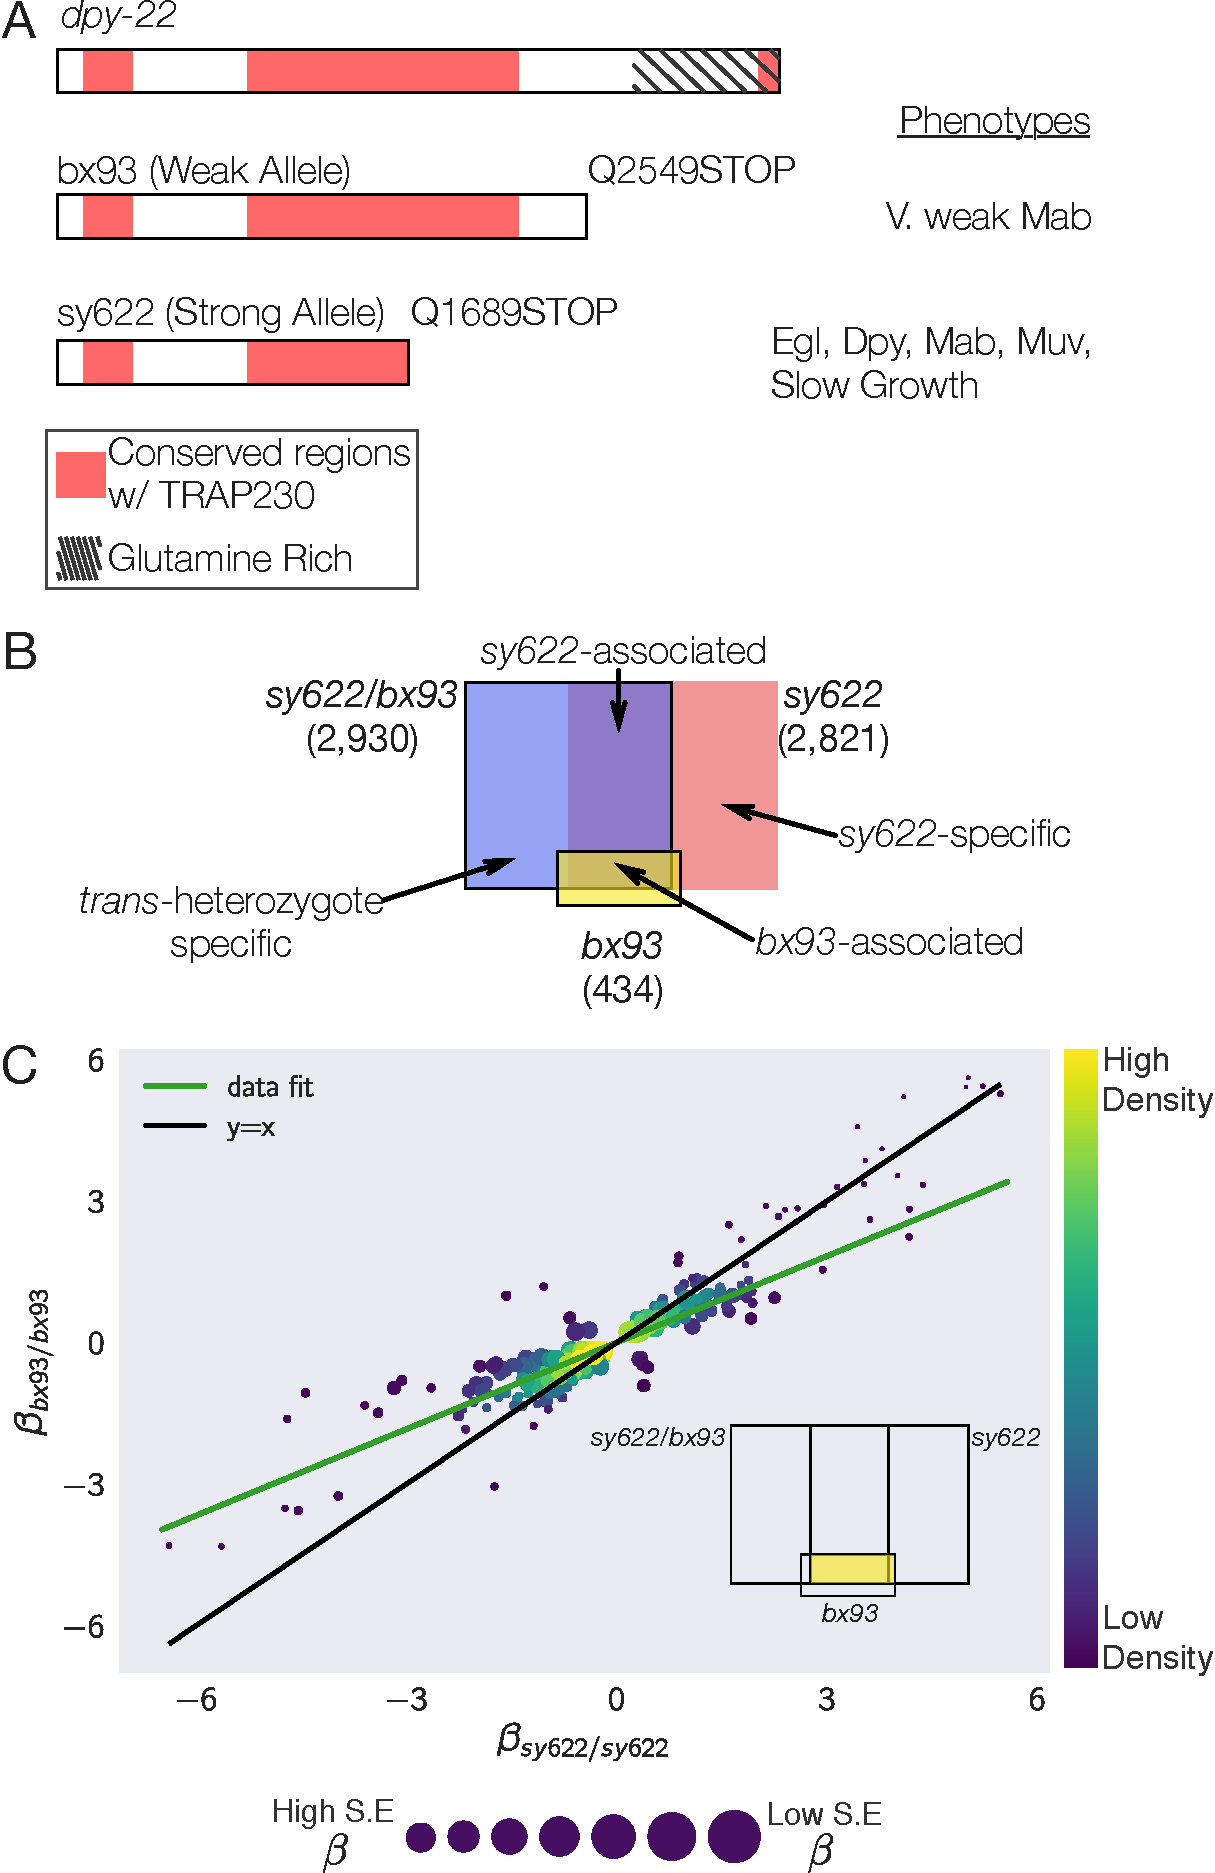
\includegraphics[width=0.5\textwidth]{../figs/dpy22_allele_comparison.pdf}
  \caption{
    The \gene{dpy-22} allelic series, consisting of two amino acid truncations,
    is amenable to study by transcriptomic phenotypes. \textbf{A}. Diagram of
    the \gene{dpy-22} gene and the \emph{bx93} and \emph{sy622} alleles.
    \textbf{B}. Venn diagram of the genotypes we sequenced: A \emph{bx93}
    homozygote, an \emph{sy622} homozygote and a \emph{bx93/sy622}
    trans-heterozygote. \textbf{C}. Genes that are commonly differentially
    expressed in both homozygotes typically change in the same direction, and
    they tend to change by 30\% less in the \emph{bx93} (weak allele) homozygote
    than in the \emph{sy622} (strong allele) homozygote. Inset shows the subset
    of genes plotted on the diagram.
    }
\label{fig:dpy22}
\end{figure}


\subsection*{The \emph{trans}-heterozygote of \gene{dpy-22} strong and weak
             alleles allows the identification of four phenotypic classes}
A standard method to identify whether two alleles differ quantitatively in their
activity levels or whether they are qualitatively different because each allele
has inactivated protein domains with separable functions is to generate a
\emph{trans}-heterozygote. Theoretically, if two alleles are quantitatively
different, the \emph{trans}-heterozygote will have a phenotype that is
intermediate to the two homozygote phenotypes. On the other hand, if both
alleles are inactivating distinct and separable functions of the protein, then
the \emph{trans}-heterozygote will exhibit a wild-type phenotype (intragenic
complementation). Finally, if one allele is affecting multiple separable
activities whereas the other allele is only affecting one, then the
\emph{trans}-heterozygote will exhibit the phenotype of the allele that affects
the least number of activities (i.e., one allele will exhibit dominance).

% TODO: check numbers here
We sequenced a trans-heterozygote of the \emph{bx93} and \emph{sy622} alleles
with genotype \gene{dpy-6(e14) bx93/+ sy622}. This trans-heterozygote appears
phenotypically wild-type, resembling the \emph{bx93} mutant morphologically. The
\emph{trans}-heterozygote showed \transn{} differentially expressed genes. Using
the trans-heterozygote, we were able to separate genes into four main phenotypic
classes, classifying them by what genotypes caused these genes to become
differentially expressed. One phenotypic class consisted of genes that were
differentially expressed in the \emph{sy622} homozygote as well as the
trans-heterozygote, but not in the \emph{bx93} homozygote (989 differentially
expressed genes). We called this the \emph{sy622}-associated phenotype. Another
phenotypic class consisted of 1,623 genes that were only dysregulated in the
\emph{sy622} homozygote, which we called the \emph{sy622}-specific phenotype
because it is entirely suppressed by the presence of a single copy of the
\emph{bx93} allele. We also found a trans-heterozygote-specific phenotype
consisting of 1,676 genes which is not present in either homozygote. Finally, we
defined a \emph{bx93}-associated phenotype as the set of genes dysregulated in
both the \emph{bx93} homozygote and the heterozygote, consisting of 310
differentially expressed genes. Having defined these classes, we set out to
describe their properties.

We asked whether these classes behaved differently within a homozygote.
Specifically, we wanted to know whether the \emph{sy622}-specific, the
\emph{sy622}-associated and the \emph{bx93}-associated phenotypes were different
in the magnitude of their perturbations or whether these subsets behaved as if
they had been randomly selected from the set of differentially expressed genes
in the \emph{sy622} homozygote (see Fig.~\ref{fig:classes}). We found that that
the \emph{bx93}-associated phenotype had the greatest magnitude of perturbations
of the three classes (mean, median and maximum). The \emph{sy622}-associated
phenotype had a smaller range of perturbations compared to the
\emph{bx93}-associated phenotype (95th percentiles: 3.3 versus 4.2,
respectively), and a statistically smaller mean (1.3 vs 0.99, respectively, $p <
10^{-5}$, non-parametric boostrap). The \emph{sy622}-specific phenotype had the
smallest mean of all (0.9, $p < 10^{-5}$ compared with \emph{bx93}-associated
phenotype, and $p = 0.01$ compared with the \emph{sy622}-associated phenotype).
The medians are almost identical between the \emph{sy622}-specific and the
\emph{sy622}-associated phenotypes, which indicates that the small difference in
the means of these two distributions is primarily driven by the longer tail of
the \emph{sy622}-associated phenotype. In conclusion, the \emph{bx93}-associated
phenotypic class contains those genes that are most sensitive to loss of function
in \protein{dpy-22}.


\begin{figure}
  \centering{}
  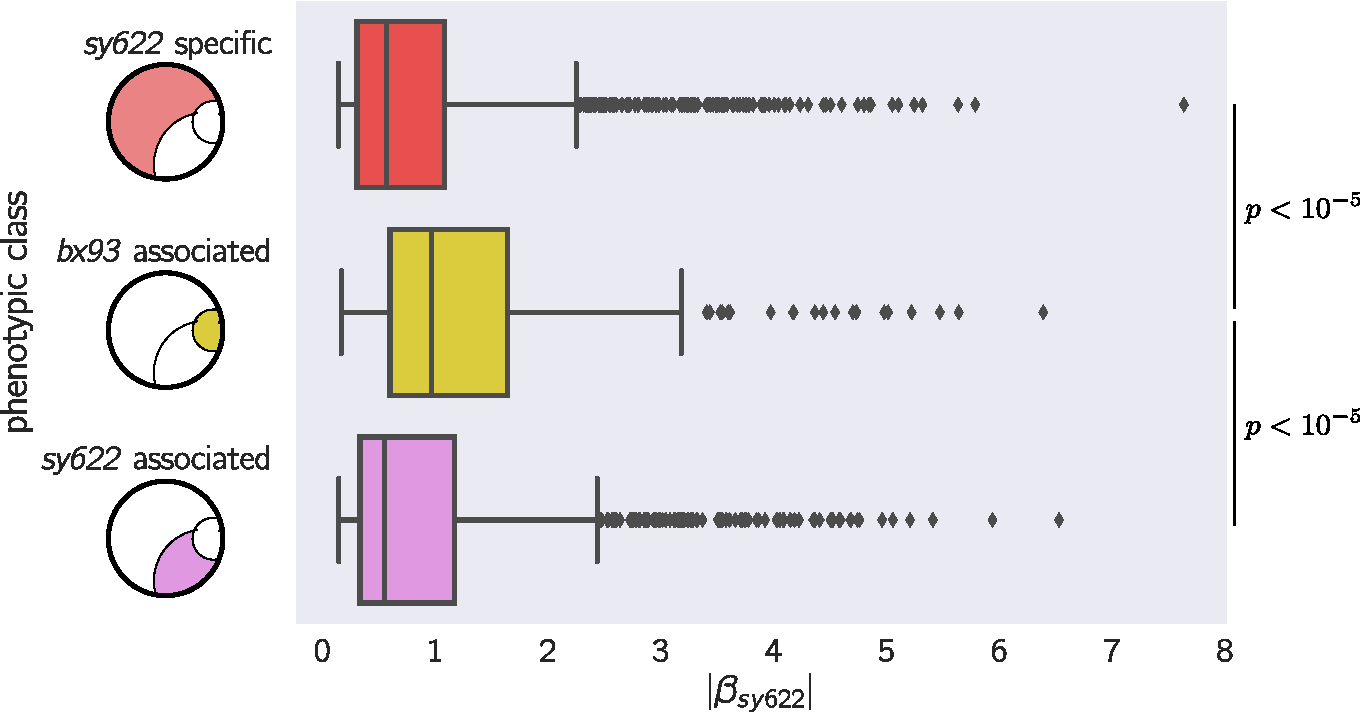
\includegraphics[width=.7\textwidth]{../figs/dpy22_classes.pdf}
  \caption{
    Within the \emph{sy622} homozygote mutant, different phenotypic classes have
    statistically different perturbation distributions. Genes that are
    \emph{sy622}-specific have a different perturbation distribution compared to
    genes that are \emph{bx93}-associated or \emph{sy622}-associated. The lines
    within the boxes show the 25, 50, and 75 percentiles. Whiskers show the rest
    of the plot, except for outliers (diamonds). Insets show what genotypes each
    gene class is expressed in, but the magnitude of the perturbation plotted
    always corresponds to the \emph{sy622} mutant. The means of each
    distribution were all statistically different from each other, as assessed
    by a non-parametric bootstrap test. The \emph{sy622}-specific and the
    \emph{sy622}-associated distributions are very similar to each other, and
    the (small) difference in the means is the result of the heavier tail of the
    \emph{sy622}-associated distribution. Notice that the x-axis,
    $|\beta_{sy622}|$, is in log-units.
  }
\label{fig:classes}
\end{figure}

\subsection*{Dominance can be quantified}
We reasoned that if one allele was dominant over the other in the heterozygote,
then plotting the $\beta$ coefficients in the homozygote of the dominant allele
versus the heterozygote should lead to a slope of 1. Deviations from a slope
with magnitude equal to unity should therefore be interpreted as deviations from
a standard dominant-recessive model. When expression in a trans-heterozygote
is intermediate between the two homozygotes, this suggests a co-dominance regime
where both alleles are contributing to the phenotype in a weighted fashion.

% TODO: Cite let-23 allelic series paper
Dominance relationships between alleles are phenotype-specific. In other
words, an allele can be dominant over another for one phenotype, yet not for
others. A classical example is the \gene{let-23} allelic series---nulls of
\gene{let-23} are recessive lethal (Let) and presumably also recessive vulvaless
(Vul) relative to the wild-type allele. The \emph{sy1} allele of
\gene{let-23} is viable dominant relative to null alleles, but is recessive
Vul~\cite{} to the wild-type allele. Above, we postulated that there are four
phenotypic classes, three of which are perturbed in the \emph{sy622} homozygote.
If these classes are indeed modular phenotypes, then the dominance relationships
within each class should be the same from gene to gene. In other words, a single
dominance coefficient should be sufficient to explain the gene expression in the
trans-heterozygote for every gene within a class.

\subsubsection*{The \emph{bx93} allele is dominant over the \emph{sy622} for the
             \emph{bx93}-associated phenotype}

We explored how expression levels changed within the \emph{bx93}-associated
phenotypic class between the homozygotes and the heterozygote. We selected the
genes within the \emph{bx93}-associated phenotypic class, and plotted the
$\beta$ coefficients of these genes in the \emph{bx93} allele against the
coefficients in the heterozygote. The coefficients fell along a line with slope
of 1.1, indicating that the \emph{trans}-heterozygote has a strong resemblance
to the \emph{bx93} homozygote, although on average its phenotype is 10\% worse
(see SIXXX).

The close resemblance of the \emph{bx93} levels to the trans-heterozygote levels
suggested that the \emph{bx93} is dominant over the \emph{sy622} allele. To
quantify this dominance, we implemented and maximized a Bayesian model. Briefly,
we asked whether there was a linear combination of the $\beta$ coefficients
of each homozygote that would predict the observed $\beta$ values of the
heterozygote, subject to the constraint that the coefficients added up to 1.
Our results suggested that the \emph{bx93} allele was responsible for
$80\% \pm 1\%$ of the gene expression phenotypes of the trans-heterozygote.
We wanted to explore how well this model explained the data. We reasoned that
if this was a modular phenotype, then it should be possible to plot the predicted
$\beta$ values against the observed $\beta$ values of the heterozygote using
this coefficient. If the model fit well, we expected to observe a clearly linear
relationship between both axes. In particular, we should not observe systematic
deviations from this model. The plot revealed that the results fit remarkably
well, furthering the case that the \emph{bx93}-associated class indeed constitutes
a modular phenotype (see Figure~\ref{fig:transhet}).

\begin{figure}
  \centering{}
  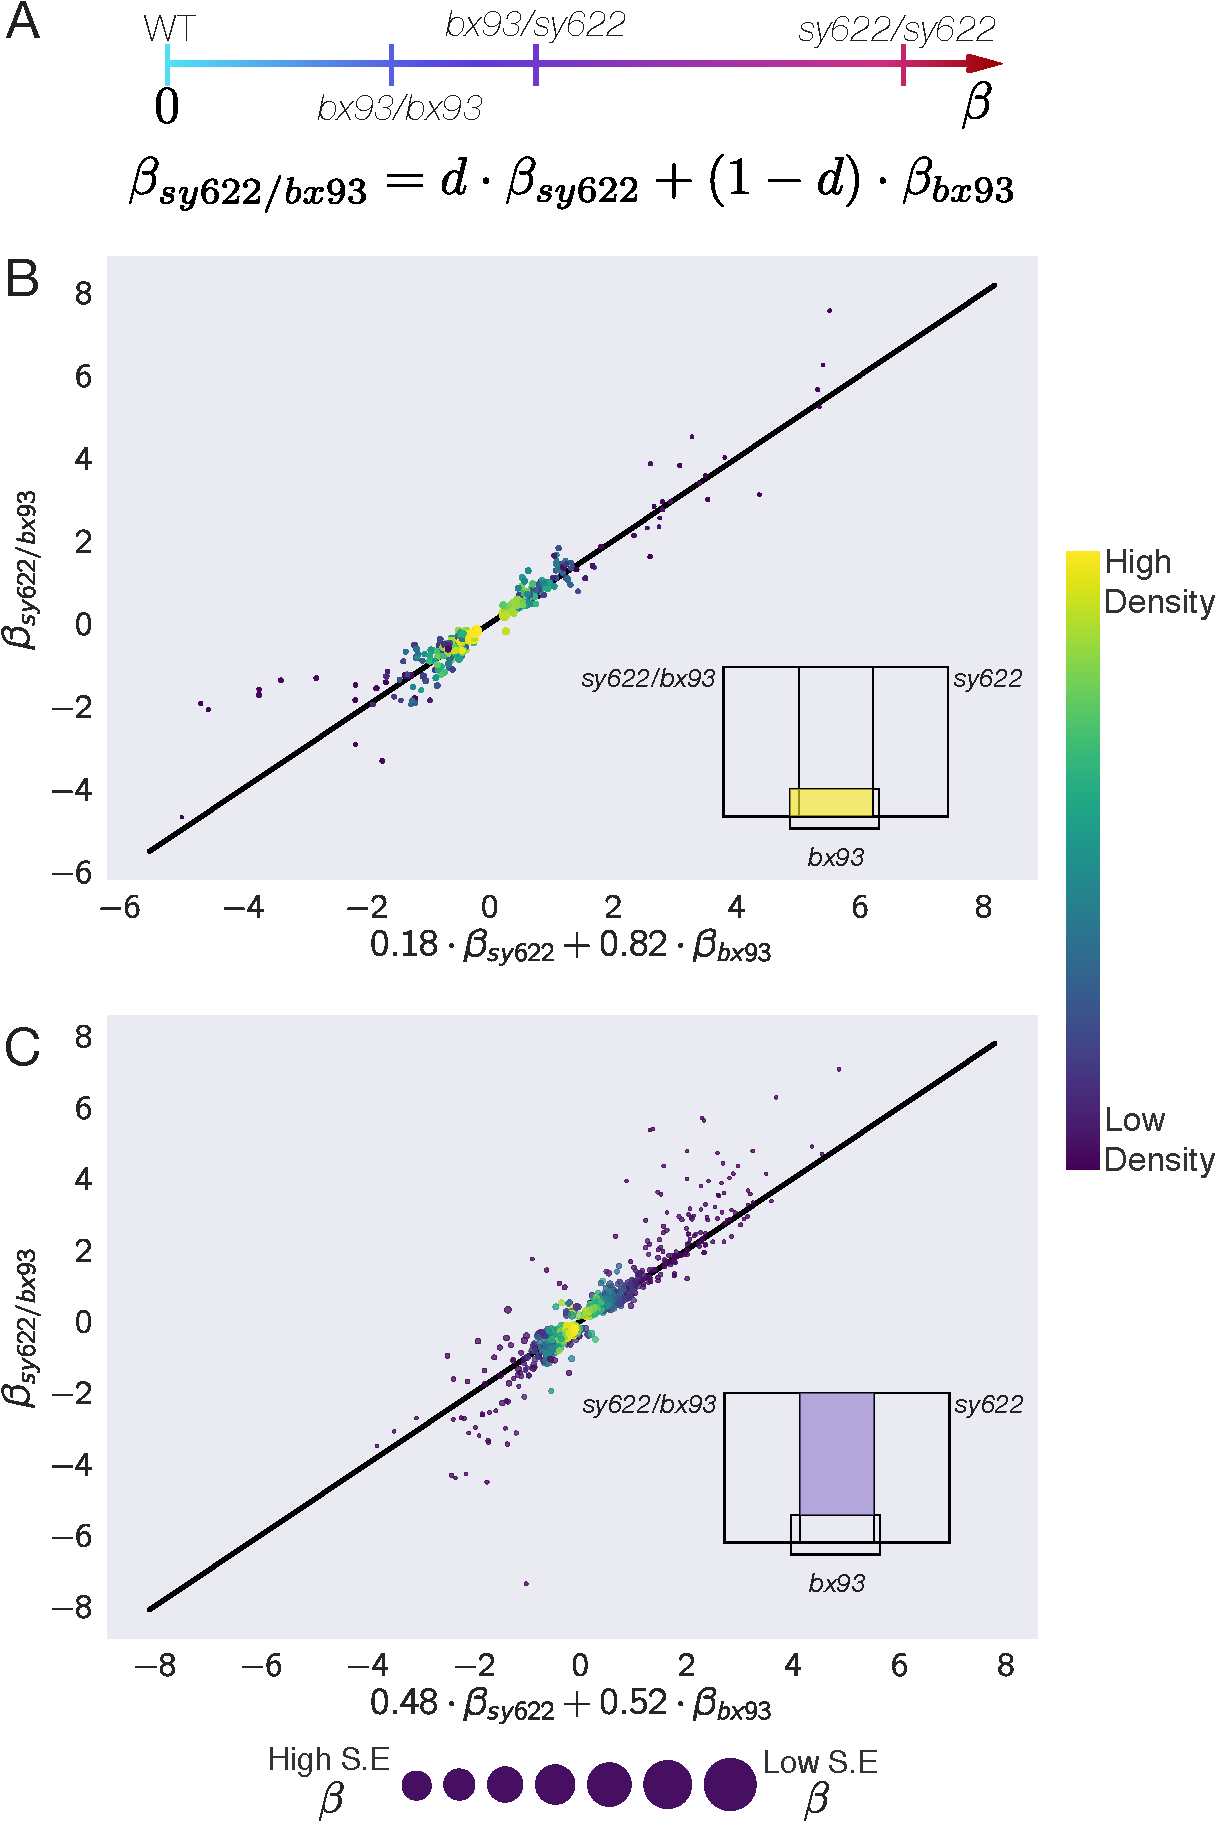
\includegraphics[width=0.5\textwidth]{../figs/dominance_classes.pdf}
  \caption{
    Alleles have a single dominance behavior for modular phenotypes.
    \textbf{A}. Schematic explaining codominance. The closer the
    trans-heterozygote is to one of the homozygotes, the more dominant the allele
    corresponding to that homozygote is considered to be. Codominance is only
    valid when the heterozygote has a phenotype between the two alleles being
    studied. Dominance is phenotype-specific, so two alleles can share different
    dominance relationships for different phenotypes.
    \textbf{B}.
    The \emph{bx93} allele is dominant over
    \emph{sy622} for the expression level of genes that fall into the
    \emph{bx93}-associated class. The \emph{bx93} is 80\% dominant over the
    \emph{sy622} allele.
    \textbf{C}. The \emph{sy622} is co-dominant with the
    \emph{bx93} allele for the expression level of genes that fall into the
    \emph{sy622}-associated class. Genes within this class show attenuated
    perturbations in the trans-heterozygote relative to the \emph{sy622}
    homozygote but do not show full complementation by the \emph{bx93} allele,
    even though the \emph{bx93} allele shows wild-type expression at these loci.
    X-axes are the predicted $\beta$ values for each subset in heterozygote
    using the data from both homozygotes.
    The dominance coefficient was estimated
    via maximum likelihood estimates on the datasets.
    Y-axes show the observed $\beta$ values for each subset in the heterozygote.
    Insets show the subset of genes plotted in each graph.
    }
\label{fig:transhet}
\end{figure}


\subsubsection*{The \emph{sy622}-associated phenotype is attenuated by the presence
            of \emph{bx93} in the trans-heterozygote}
We also wanted to know whether the \emph{sy622}-associated phenotype showed
differences depending on genotypic context. The \emph{sy622}-associated genes
are genes that are differentially expressed in the \emph{sy622} homozygote or
the trans-heterozygote, but not the \emph{bx93} homozygote. Genes in this group
showed a 23\% reduction in the magnitude of their perturbations in the
heterozygote compared to the homozygote (see
SIXXX). Therefore, these genes are attenuated by
the presence of a single copy of the \emph{bx93} allele. To determine the
relative dominance of \emph{bx93} and \emph{sy622}, we implemented the same model
as above and found the coefficient that maximized the probability of observing
the data. We found that \emph{bx93} and \emph{sy622} are almost perfectly
codominant. \emph{sy622} has a dominance coefficient of $48\% \pm 1\%$.
This behavior is qualitatively different from genes in the
\emph{bx93}-associated phenotypic class, where \emph{bx93}
was 80\% dominant. Finally, the behaviors of both of these classes are distinct
from the behavior of genes in the \emph{sy622}-specific class, which show
differential expression in a \emph{sy622} homozygote, but this dysregulation is
complemented by the \emph{bx93} allele (by definition, the dominance coefficient
associated with \emph{bx93} must be 1 for this class). This establishes that
alleles can have differences in dominance for different phenotypic classes at
the gene expression level.

\subsection*{Insights into the physiology of \emph{sy622} homozygotes}
Whereas the \emph{sy622} homozygote is strongly phenotypic (see
Fig.~\ref{fig:dpy22}), the \emph{bx93} is almost entirely wild-type. Since the
trans-heterozygote also appears grossly wild-type, we hypothesized that the
\emph{sy622}-specific phenotypic class was associated with the macroscopic
phenotypes visible in the \emph{sy622} allele. To better understand this
phenotypic class, we used the Wormbase Enrichment
Suite~\cite{Angeles-Albores2016,Angeles-Albores106369} to query what anatomical,
phenotypic or gene ontological terms were enriched in this gene set (see
Table~\ref{tab:enrich}).
%
% \begin{table}[tbhp]
%   \centering
%   \begin{tabular}{llrrrr}
%     \toprule{}Phenotypic class & Term & No.\ of Observed Genes & Fold-change & $-\log_{10}{q}$\\
%     \midrule{}\emph{sy622}-specific & Intestine & 764 & 1.3 & $12$\\
%     \emph{sy622}-specific & Intestinal muscle  & 42 & 2.0 & $4$\\
%     \emph{sy622}-specific & PVD & 362 & 1.2 & $3$\\
%     \emph{sy622}-specific & Muscular system & 639 & 1.2 & $7$\\
%     \emph{sy622}-specific & Severe pleiotropic defects early embryo & 32 & 2.4 & $4$\\
%     \emph{sy622}-specific & Rachis absent & 24 & 2.5 & $4$\\
%     \emph{sy622}-specific & Meiosis defective early embryo & 21 & 2.3 & $3$\\
%     \emph{sy622}-specific & Collagen trimers & 44 & 7.7 & $25$\\
%     \emph{sy622}-specific & Muscle cell development & 29 & 5.7 & $13$\\
%     \emph{sy622}-specific & Contractile fibers & 33 & 5.2 & $14$\\
%     \emph{sy622}-specific & Oviposition & 44 & 3.6 & $12$\\
%     \emph{bx93}-specific & Intestine &  &  & $-$\\
%     \emph{bx93}-specific & pm3/5 & 4 & 5.6 & $2$\\
%     \emph{bx93}-specific & Dauer constitutive & 7 & 4.9 & $2$\\
%     \emph{bx93}-specific & Dauer metabolism & 18 & 2.5 & $2$\\
%     \emph{bx93}-specific & Glucuronosyltransferase activity & 9 & 22.0 & $9$\\
%     \emph{bx93}-specific & Monocarboxylic acid catabolic process & 5 & 11.6 & $4$\\
%     \emph{bx93}-specific & Lytic vacuole & 5 & 10.1 & $4$\\
%     \bottomrule{}
%   \end{tabular}
%   \caption{
%     List of enriched terms for the \emph{sy622}-specific and \emph{bx93}-specific
%     phenotypic classes. Fold-change is calculated relative to the expected number
%     of observations for any given term under the null hypothesis that terms are
%     drawn at random. Q-values are calculated using a hypergeometric model and
%     adjusted via a Benjamini-Hochberg algorithm. Q-values shown are rounded to
%     the nearest power of 10 for simplicity.
%   }
% \label{tab:enrich}
% \end{table}
%
\begin{table}[tbhp]
  \centering
  \begin{tabular}{lcc}
    \toprule{}Term & \emph{sy622}-specific $-\log_{10}{q}$ & \emph{bx93}-associated $-\log_{10}{q}$\\
    \midrule{}Intestine & $12$ & $-$\\
    Intestinal muscle & $4$ & $<1$\\
    PVD & $3$ & $<1$\\
    Muscular system & $7$ & $<1$\\
    pm3/5 & $<1$ & $2$\\
    Severe pleiotropic defects early embryo & $4$ & $<1$\\
    Rachis absent & $4$ & $<1$\\
    Meiosis defective early embryo & $3$ & $<1$\\
    Dauer constitutive & $<1$ &$2$\\
    Dauer metabolism  & $<1$ &$2$\\
    Collagen trimers  & $25$ & $<1$\\
    Muscle cell development & $13$ & $<1$\\
    Contractile fibers & $14$ & $<1$\\
    Oviposition & $12$ & $<1$\\
    Glucuronosyltransferase activity &$<1$ & $9$\\
    Monocarboxylic acid catabolic process &$<1$ & $4$\\
    Lytic vacuole & $<1$& $4$\\
    \bottomrule{}
  \end{tabular}
  \caption{
    List of enriched terms for the \emph{sy622}-specific and
    \emph{bx93}-specific phenotypic classes. The \emph{sy622}-specific and the
    \emph{bx93}-associated columns show $-\log_{10}{q}$ for each term. Q-values
    are calculated using a hypergeometric model and adjusted via a
    Benjamini-Hochberg algorithm. Q-values shown are rounded to the nearest
    power of 10 for simplicity. $<1$ implies that the q-value did not pass the
    significance threshold.
  }
\label{tab:enrich}
\end{table}

The \emph{sy622}-specific phenotypic class was enriched for genes expressed in
the intestine and intestinal muscle. We also found enrichment in cell-types that
could reasonably be associated with egg-laying defects, namely the PVD neuron,
and the muscular system. Phenotype ontology enrichment revealed that the
\emph{sy622}-specific phenotypic class was enriched for terms associated with
embryonic lethality and small brood size, such as severe pleiotropic defects in
the early embryo, oocytes lack nucleus, rachis absent and meiosis defective in
the early embryo. Gene ontology enrichment showed that the \emph{sy622}-specific
phenotype was enriched in collagen trimers, muscle cell development, contractile
fibers and oviposition. In contrast, the \emph{bx93}-specific phenotypic class
does not enrich identical terms. Rather, the \emph{bx93}-specific class shows
enrichment for genes expressed in the intestine and pharyngeal muscle cells, pm3
and pm5. It shows enrichment of genes associated with dauer constitutive and
dauer metabolism phenotypes, and the gene ontology enrichment primarily reflects
terms associated with metabolism, such as glucuronosyltransferase activity,
monocarboxylic acid catabolic process, and lytic vacuole.

\section*{Conclusions}
\subsection*{Gain-of-function and loss-of-function alleles can lead to different
             transcriptomic states.}
We sequenced a weak gain-of-function (\emph{n1046gf}) and a strong
loss-of-function (\emph{n2021}) allele of Ras, with the expectation that these
alleles would affect the same set of genes in opposite ways, because the
gain-of-function allele is thought to signal more than the wild type, whereas
the loss-of-function does not signal at all. Contrary to our expectations, we
find that these gene sets are substantially disjoint with a relatively small
overlap. Within this overlap, we find that genes that are commonly
differentially expressed in homozygotes of either allele tend to show changes of
exactly the same magnitude and direction. In other words, the effect of
loss-of-function and gain-of-function for these genes is exactly the same.
Moreover, we find that for a smaller population of genes where loss-of-function
and gain-of-function have opposing effects on gene expression, the magnitude of
change is also the same. We considered various mechanisms that could generate
these patterns.

We considered a scenario where the \gf{} signals constitutively through pathways
that are only sparingly used in wild-type animals. This model would predict that
the \gf{} mutant would show changes in these pathways as they are flooded with
new information through channels that are rarely used. In contrast, the \lf{}
mutant should show fewer changes in these pathways, because in this model most
of the changes are rarely in use. Thus, genes that are differentially expressed
in the \gf{} homozygote would be interpreted as genes where \ras{} is sufficient
to trigger changes in expression, and the changes in the \lf{} represent genes
where \ras{} is necessary for appropriate expression. Although this scenario
begins to explain the difference in size between the number of differentially
expressed genes in the \gf{} homozygote and the \lf{} homozygote, it does not
explain why there are genes that are differentially expressed in the \lf{}
homozygote that are not present in the \gf{}. Moreover, this model does not
explain why the STP between the \lf{} and \gf{} homozygotes is predominantly
correlated, instead of being entirely anti-correlated. Therefore, it seems
unlikely that the transcriptomes of these alleles result from a model where
\ras{} is capable of signaling through a large number of pathways but
predominantly uses only a subset.

A mechanism that could feasibly generate \letlf{}- and \letgf{}-specific effects
as well as correlated and anti-correlated effects would be to postulate that
there are four signaling states available to \rasp{}. In this model, a protein
bound to GTP constitutively can signal through a set of proteins, whereas a
protein bound to GDP signals through a different, non-overlapping pathway. A
third pathway requires GTP-to-GDP cycling at a specific average rate, such that
interfering with that cycling by stabilizing either the GTP- or GDP-bound states
has the same effect. A similar effect has been described previously for the Sec4
GTPase~\cite{}\todo{cite Peter Novick here}.

Another way to understand the effects we observed in \letlf{} and \letgf{}
mutants is by thinking of the transcriptomes of each mutant as their respective
states. Recently, transcriptome profiling has been used to identify novel states
in both single cells and whole-organisms~\cite{Villani2017}\todo{cite female
state paper}. If these transcriptomes are states, then these states are the
result of continous \ras{} activity (or inactivity) throughout the lifespan of
the animal, and reflect the proximal or immediate effects of altered \rasp{}
activity a well as compensatory changes due to altered development or life
history. This framework has the advantage that it does not \emph{a priori}
suggest that the \gf{} homozygote and \lf{} homozygote should have similar, or
even overlapping, effects.

Without many more experiments, we cannot definitively point at a mechanism. It
is possible that background mutations are contributing to the \letlf{}- and
\letgf{}-specific changes, since these mutants were identified in different
screens carried out in different labs. A rigorous methodology to exclude
background mutations would call for sequencing multiple independent lines
containing each allele. As library generation and sequencing costs fall, these
experiments will become more feasible. Even assuming that background effects are
responsible for the lack of overlap between the two mutants, the positive and
negative correlations between these two alleles raise important questions about
Ras biology. The fact that either correlation has a value with magnitude exactly
of 1 suggests the existence of circuits that monitor Ras signaling levels with
quantitative accuracy in \cel{}.

\subsection*{Loss-of-function allelic series reveal unknown functionality}
We sequenced two alleles of \gene{dpy-22} that had been previously studied and
reported to have different functionalities. Through transcriptomic profiling, we
were able to verify that \emph{sy622} has a transcriptomic phenotype that is
quantifiably worse than \emph{bx93}. This worsening manifests as an increase in
the number of differentially expressed genes in \emph{sy622} relative to
wild-type compared to the number of differentially expressed genes in
\emph{bx93}. Moreover, the genes that are commonly dysregulated in both alleles
show greater perturbations on average in the \emph{sy622} homozygote relative to
the \emph{bx93} allele (see Fig.~\ref{fig:dpy22}). Unlike the \ras{} alleles we
studied, the set of genes differentially expressed in the \emph{bx93} is
contained within the \emph{sy622} with few exceptions. We can account for most
of these exceptions by invoking a 10\% false positive rate (which was the cutoff
for our study) and a similar false negative rate.

Although a comparison between these two alleles proves fruitful in establishing
differences in phenotypic severity, this comparison alone does not allow us to
answer whether or not \emph{bx93} and \emph{sy622} act in different ways on
subsets of genes. To this end, we sequenced a trans-heterozygote of both
alleles, which allowed us to identify four phenotypic classes, which in turn are
informative about the biological effects of each allele. We found a
\emph{sy622}-specific phenotypic class for which the \emph{bx93} has a dominant
wild-type phenotype; we found a \emph{bx93}-associated phenotypic class for
which \emph{bx93} also has a dominant phenotype, but this phenotype is
definitely not wild-type. We also found a \emph{sy622}-associated class for
which \emph{sy622} and \emph{bx93} appear co-dominant. Intriguingly, we also
found a phenotype specific to the trans-heterozygote that was not present in
either homozygote. A weakness in our study is that we have limited power to
study the gene expression changes associated with the trans-heterozygote. This
phenotypic class is puzzling because \dpy{} is not known to have homotypic
interactions, which is a classical explanation for trans-heterozygote-specific
phenotypes. Moreover, since this class is specific to a single strain we cannot
rule out that this class is actually a result of a strain-specific mutation or
set of mutations. In particular, the genotype of the heterozygote includes a
mutation at the \gene{dpy-6} locus to balance the \emph{bx93} mutation. One
possibility is that the \emph{dpy-6} loss-of-function mutation is not recessive
for transcriptomic phenotypes and is responsible for the dysregulation of the
new genes observed in the heterozygote. Another possibility is that the
\emph{dpy-6} strain had a carrier mutation that fixed in the balanced strain.
Finally, it is also possible that the \emph{bx93} and the \emph{sy622} strains
had background mutations that did not have effects on their own, but when
combined generate a synthetic phenotype with themselves or with one or both of
the \gene{dpy-22} alleles. As the cost of sequencing becomes lower, and with
improved genetic engineering tools that allow the creation of background-free
mutations, it will become increasingly important to rule out these hypotheses by
sequencing additional independently derived identical alleles.

Our enrichment analysis of the \emph{sy622}-specific and the
\emph{bx93}-associated phenotypic classes revealed that they reflect
functionally distinct aspects of \dpy{} biology. The \emph{sy622}-specific class
contains genes that are associated with severe pleiotropic effects, embryonic
lethality and sterility. It also contains genes that are associated with muscle
development and function, and there is enrichment of genes expressed in the PVD
neuron. Finally, collagen trimers are also overrepresented in this gene class.
Taken together, these terms suggest that perturbing this gene class away from
the wild-type should lead to an animal that is sickly, has a small brood size
and has altered locomotion as well as altered collagen production. Indeed, the
\emph{sy622} homozygote is Dpy and Egl and RNAi against \dpy{} is known to cause
embryonic and larval lethality~\cite{}. The \emph{bx93}-associated class is
enriched in a different set of terms, which suggests that transcriptome
profiling can be used in conjunction with allelic series to separate genes into
distinct phenotypic classes that are biologically relevant. Specifically, for
the \emph{sy622} and the \emph{bx93} alleles, we can rule out that these alleles
form a qualitative allelic series, since such a series should not exhibit a
dosage-dependent phenotype (the \emph{sy622}-associated class). However, it is
possible that \emph{sy622} and \emph{bx93} represent a mixed
quantitative-qualitative series, because we found phenotypic classes where
\emph{bx93} complemented \emph{sy622}, \emph{bx93} was dominant over
\emph{sy622} and where \emph{sy622} was co-dominant with or partially dominant
over \emph{bx93}.

\todo[inline]{Add self-citations below.}
Allelic series are a cornerstone of genetic analyses. Classically, these series
have been important to understand multiple aspects of a gene by comparing and
contrasting the properties of different alleles in homozygotes as well as
heterozygotes. Due to their sensitivity and quantitative nature, transcriptomic
phenotypes represent an exciting new phenotype with which to study these series.
Here, we have shown that transcriptomic phenotypes can quickly and easily
partition gene sets into phenotypic classes that have different statistical and
physiological properties. Recents developments in the fields of transcriptomics
have shown that expression profiles can be used for genetic pathway
analysis~\cite{} as well as for the identification of novel cellular or animal
states~\cite{}. In particular, single-cell sequencing has shown great
potential as a tool because it can help understand transcriptional heterogeneity
at the cellular level, but also because random screens can be used to
simultaneously knock out random combinations of genes and infer genetic
interactions~\cite{} (Perturb-Seq). Here, we highlight the importance of
understanding allelic diversity towards understanding distinct biological
properties of the genes in question. In addition to sequencing great numbers of
cells to understand cell-cell heterogeneity and diversity, we should also
sequence diverse alleles in order to better understand genotype-genotype
heterogeneity.


\section*{Acknowledgements}
This work was supported by HHMI with whom PWS is an investigator and by the
Millard and Muriel Jacobs Genetics and Genomics Laboratory at California
Institute of Technology. All strains were provided by the CGC, which is funded
by NIH Office of Research Infrastructure Programs (P40 OD010440). This article
would not be possible without help from Dr.\ Igor Antoshechkin and Dr.\ Vijaya
Kumar who performed the library preparation and sequencing.

%This is where your bibliography is generated.
\bibliography{citations}

%This defines the bibliographies style.
\bibliographystyle{naturemag}

\end{document}
